\documentclass[11pt]{article}
\usepackage[margin=1in]{geometry}
\usepackage{graphicx}
\usepackage{booktabs}
\usepackage{amsmath}
\usepackage{siunitx}
\usepackage[hidelinks]{hyperref}
\usepackage{xcolor}

\newcommand{\Rp}{R_{\rm p}}
\newcommand{\Mdot}{\dot{M}}
\newcommand{\FXUV}{F_{\rm XUV}}
\newcommand{\Fo}{F_{0}}
\newcommand{\HeTS}{\mathrm{He}\,2^{3}S}

\title{WASP-52b: EXHALE Atmospheric-Escape Model vs.\ He\,10830 and H$\alpha$ Observations}
\author{EXHALE modeling notes}
\date{Last updated: 2026-06-17}

\begin{document}
\maketitle

\begin{abstract}
We model the upper atmosphere and escaping wind of the hot Jupiter WASP-52b with
\texttt{EXHALE} (the extended ATES code) and compare the synthetic He\,\textsc{i}
10830 and H$\alpha$ transit transmission spectra against published observations.
The setup follows Yan et al.\ (2022): the stellar XUV/FUV spectral energy
distribution is taken from $\epsilon$\,Eri (MUSCLES) scaled to the planet's orbit,
the lower boundary is pressure-anchored at 1\,$\mu$bar, and the full Roche (tidal)
potential is used. The steady-state mass-loss rates reproduce Yan et al.\ (2022)
to within $\sim$10\% at every XUV level. The He\,10830 absorption is shown to be
governed by the metastable $\HeTS$ population: with the physically motivated
$L_1$-truncated domain, a He-poor composition (H/He\,$\simeq$\,98/2) and the
best-fit XUV flux ($0.5\,\Fo$), the model reproduces the observed He\,10830 line
depth ($\sim$4\% vs.\ $\sim$3.4\%). An extended $10\,\Rp$ domain over-predicts the
absorption by $3$--$10\times$ because of an unphysical $\HeTS$ tail beyond $L_1$.
The H$\alpha$ prediction is not trusted because the Ly$\alpha$ radiative transfer
that sets the $n=2$ hydrogen population is not solved here.
\end{abstract}

\section{Target and goal}
WASP-52b is a low-density hot Jupiter on a 1.75\,d orbit around an active K2V star;
excess absorption has been detected in both He\,10830 (Kirk et al.\ 2022) and
H$\alpha$ (Chen et al.\ 2020). Our goal is to compute a \emph{base} \texttt{EXHALE}
model (no fitting) and overplot the synthetic He\,10830 and H$\alpha$ transmission
spectra on the observations. The adopted planet/star parameters
(Table~\ref{tab:params}) match Yan et al.\ (2022), whose hydrodynamic code
(Yang \& Guo 2018) we use as the physics reference.

\begin{table}[h]
\centering
\caption{Adopted WASP-52 / WASP-52b parameters (Yan et al.\ 2022).}
\label{tab:params}
\begin{tabular}{lll}
\toprule
Quantity & Value & Note \\
\midrule
Stellar mass $M_\star$        & $0.87\,M_\odot$   & K2V \\
Stellar radius $R_\star$      & $0.79\,R_\odot$   & \\
Stellar $T_{\rm eff}$         & $5000$\,K         & for the Balmer continuum \\
Planet mass $M_{\rm p}$       & $0.46\,M_{\rm J}$ & \\
Planet radius $\Rp$           & $1.27\,R_{\rm J}$ & base radius \\
Equilibrium temperature $T_0$ & $1304$\,K         & $=$ base temperature \\
Orbital distance $a$          & $0.0272$\,au      & \\
He/H number ratio             & $0.087$ (solar) \dots $0.005$ & scanned (\S\ref{sec:scan}) \\
Base pressure                 & $1\,\mu$bar       & $\to n_0=5.56\times10^{12}\,\mathrm{cm^{-3}}$ \\
\bottomrule
\end{tabular}
\end{table}

\section{Stellar input spectrum}
WASP-52's XUV spectrum is unobserved, so following Yan et al.\ (2022) we use the
$\epsilon$\,Eri spectrum from the MUSCLES Treasury Survey (France et al.\ 2016),
scaled from Earth to the planet's orbit by $(d_{\epsilon\,\rm Eri}/a)^2$ with
$d_{\epsilon\,\rm Eri}=3.212$\,pc. The scaling reproduces Yan's fiducial values:
\begin{center}
\begin{tabular}{lll}
\toprule
Band & This work & Yan et al.\ (2022) \\
\midrule
$\FXUV$ (1--912\,\AA)      & $3.44\times10^{4}\,\mathrm{erg\,cm^{-2}\,s^{-1}}$ & $3.42\times10^{4}$ \\
$\beta_m=F(1\text{--}100)/F(1\text{--}912)$ & $0.218$ & $0.22$ \\
FUV/NUV (912--2600\,\AA)   & $2.63\times10^{5}\,\mathrm{erg\,cm^{-2}\,s^{-1}}$ & $\sim2.6\times10^{5}$ \\
\bottomrule
\end{tabular}
\end{center}
The FUV/NUV band photoionizes the He\,$2^3S$ metastable level and is therefore
essential for the He\,10830 prediction. \texttt{EXHALE} reads the two-column
(wavelength, flux) SED file directly and integrates it for the band luminosities
and the frequency-dependent photoionization/heating rates.

\paragraph{Flux normalization (important).}
Yan et al.\ divide the substellar $\FXUV$ by 4 to account for redistribution over
the sphere, defining $\Fo\equiv\FXUV/4=8542\,\mathrm{erg\,cm^{-2}\,s^{-1}}$, and
explore $0.25$--$8\,\Fo$. In \texttt{EXHALE} the SED is the full substellar flux
and the 2-D approximation ``Rate/2 + Mdot/2'' multiplies it by $0.5$ inside the
simulation. Hence our $0.25\times$, $0.5\times$, $1.0\times$ fiducial SED map to
Yan's $0.5\,\Fo$, $1\,\Fo$, $2\,\Fo$ respectively. Yan's best fit to the
observations is $0.5\,\Fo$, i.e.\ our $0.25\times$ SED.

\section{Numerical setup}
The lower boundary is pressure-anchored at 1\,$\mu$bar (\texttt{Base BC: pressure
1.0}), giving $n_0=P/(k_BT_0)=5.56\times10^{12}\,\mathrm{cm^{-3}}$, identical to
Yan's base condition. The He\,$2^3S$ (metastable) network is enabled
(\texttt{Include He23S? True}); trace metals (C/N/O$+$Mg/Ca/Na/Fe) are optionally
added via \texttt{metals.inp}. Convergence uses the two-stage PLM$\to$WENO3 march
with a du-keyed hand-off to the Newton/JFNK solver. The automatic initial-condition
selector (\texttt{IC mode: auto}) chooses a transonic wind seed (the interior cold
sonic point sits at $r_c\simeq2.42\,\Rp$).

\paragraph{Domain: tidal potential, two outer boundaries.}
The full Roche potential along the substellar axis is used in all runs. We compare
two outer boundaries:
\begin{itemize}
\item \textbf{Extended ($10\,\Rp$):} matching Yan's domain extent. This required a
  one-line extension so that an explicit \texttt{Outer radius} is honored in Roche
  mode while keeping the tidal terms (documented in the user manual / update log).
\item \textbf{$L_1$-truncated ($\simeq2.53\,\Rp$):} the default Roche behavior,
  truncating at the inner Lagrange point where the effective gravity vanishes.
\end{itemize}
The tidal force is treated identically to Yan/Yang: the momentum equation carries
gravity $+$ stellar tide $+$ centrifugal terms. The escape-energy drop from $\Rp$
to $L_1$ in the full Roche form (0.431 in $GM_{\rm p}/\Rp$ units) agrees with the
Erkaev et al.\ (2007) reduced form $K(\lambda)=1-3/2\lambda+1/2\lambda^3=0.428$ to
$0.6\%$ for WASP-52b, so the two tidal prescriptions are effectively equivalent here.

\section{Mass-loss validation}
\label{sec:mdot}
At matched XUV flux the \texttt{EXHALE} steady-state mass-loss rates reproduce Yan
et al.\ (2022, their Table~4) to within $\sim$10\% (Table~\ref{tab:mdot}). This
confirms that the wind hydrodynamics and energy balance are consistent with the
reference code; differences in the line predictions below are therefore not driven
by the mass loss.

\begin{table}[h]
\centering
\caption{Steady-state mass-loss rate $\log_{10}\Mdot$ [g\,s$^{-1}$] vs.\ Yan et
al.\ (2022) Table~4 ($\beta_m=0.22$). Our SED multiple maps to Yan's $\Fo$
multiple as noted.}
\label{tab:mdot}
\begin{tabular}{llcc}
\toprule
Composition & Flux & EXHALE & Yan (2022) \\
\midrule
H/He $=$ 92/8 & $1\,\Fo$ (our $0.5\times$) & 11.69 & 11.70 \\
H/He $=$ 92/8 & $2\,\Fo$ (our $1.0\times$) & 11.93 & 11.96 \\
H/He $=$ 98/2 & $1\,\Fo$ (our $0.5\times$) & 11.74 & 11.69 \\
H/He $=$ 98/2 & $2\,\Fo$ (our $1.0\times$) & 11.98 & 11.95 \\
H/He $=$ 92/8 & $0.5\,\Fo$ (our $0.25\times$) & 11.47 & 11.44 \\
H/He $=$ 98/2 & $0.5\,\Fo$ (our $0.25\times$) & 11.49 & 11.41 \\
\bottomrule
\end{tabular}
\end{table}

\section{He\,10830: extended domain over-predicts}
\label{sec:he10rp}
With the $10\,\Rp$ extended domain the model He\,10830 excess absorption is
$15$--$50\%$, far above the observed $\sim$3.4\% (Fig.~\ref{fig:cmp10rp}, left).
The H$\alpha$ panel is shown but is not trusted (see \S\ref{sec:halpha}).

\begin{figure}[h]
\centering
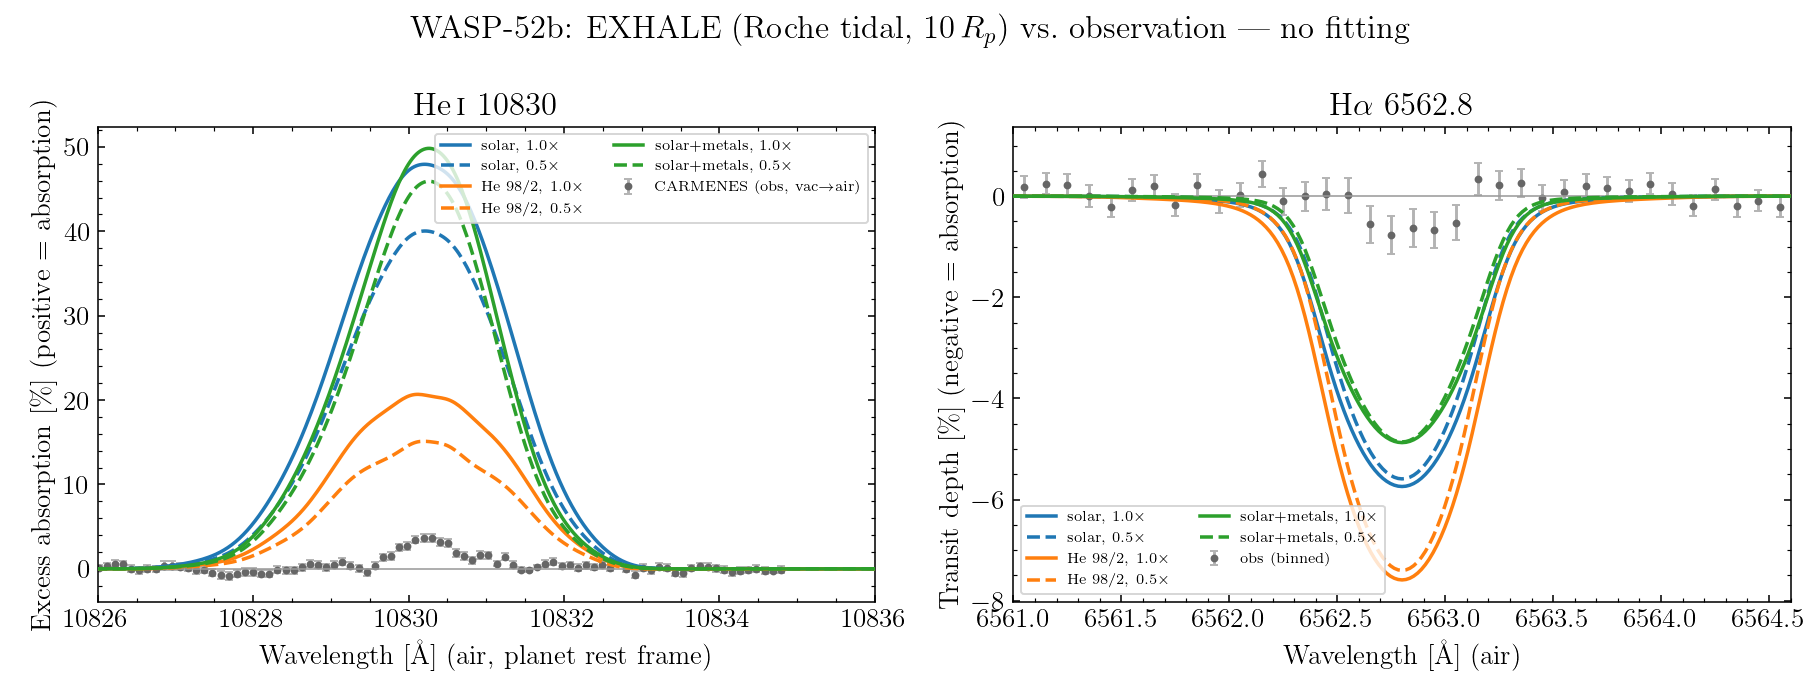
\includegraphics[width=\textwidth]{compare_WASP-52b.png}
\caption{Extended-domain ($10\,\Rp$) model vs.\ observations. He\,10830 (left,
excess absorption, positive\,$=$\,absorption; observation converted vacuum$\to$air)
and H$\alpha$ (right, transit spectrum, negative dip\,$=$\,absorption). Color
$=$ composition, line style $=$ XUV level. The model over-predicts He\,10830 by
$3$--$10\times$.}
\label{fig:cmp10rp}
\end{figure}

\paragraph{Diagnosis: the metastable $\HeTS$ tail.}
The over-prediction is \emph{not} a mass-loss or flux-normalization error (the
$\Mdot$ matches Yan, \S\ref{sec:mdot}). It arises from the spatial distribution of
the $\HeTS$ population. In the steady state
\begin{equation}
\frac{n(\HeTS)}{n_{\rm He^+}} \;\simeq\; \frac{\alpha_3\,n_e}{\Phi_3 + A_{31}
   + (q_{31a}+q_{31b})n_e + Q_{31}n_{\rm H}},
\end{equation}
where $\alpha_3$ is the He$^+$ recombination into $2^3S$, $\Phi_3$ the FUV
photoionization rate, $A_{31}=1.27\times10^{-4}\,\mathrm{s^{-1}}$ the radiative
decay, and $q_{31},Q_{31}$ the electron / hydrogen collisional sinks. We verify
$\Phi_3=0.061\,\mathrm{s^{-1}}$ (at $1\,\Fo$) directly from the SED and the NIST
cross section, consistent with the FUV flux above. In the cool, rarefied outer wind
the collisional sinks vanish, leaving photoionization as the only sink; the ratio
$n(\HeTS)/n_{\rm He^+}=\alpha_3 n_e/\Phi_3$ then \emph{rises} outward and the
$\HeTS$ density stays nearly flat from $2$ to $5\,\Rp$. Because the transit depth is
weighted by the impact parameter ($\propto r^2$), this sustained outer tail
dominates: \textbf{72\% of the He absorbing column comes from $r>L_1$ ($2.53\,\Rp$).}
Beyond $L_1$ the gas is Roche-unbound and physically funnels through $L_1$ rather
than forming a complete spherical shell, so the 1-D spherical treatment to
$10\,\Rp$ over-counts the absorption.

\section{He\,10830: $L_1$-truncated domain reproduces the observation}
\label{sec:heL1}
Truncating the domain at $L_1$ removes the unphysical outer tail and brings the
He\,10830 depth into agreement with the data (Table~\ref{tab:hedepth},
Fig.~\ref{fig:cmpL1}). At the best-fit flux ($0.5\,\Fo$) and a He-poor composition
(H/He\,$=$\,98/2), the model gives $3.9\%$ vs.\ the observed $\sim$3.4\%. The solar
(92/8) composition remains too strong ($7.4\%$), independently confirming Yan's
conclusion that a high H/He ratio is required to match the He\,10830 line.

\begin{table}[h]
\centering
\caption{He\,10830 line-center excess absorption [\%] for the extended ($10\,\Rp$)
and $L_1$-truncated domains. Observed $\sim$3.4\%.}
\label{tab:hedepth}
\begin{tabular}{llcc}
\toprule
Flux & Composition & $10\,\Rp$ & $L_1$-trunc. \\
\midrule
$0.5\,\Fo$ & 92/8 (solar)   & 30.6 & 7.4 \\
$0.5\,\Fo$ & 98/2 (He-poor) & 11.2 & \textbf{3.9} \\
$1\,\Fo$   & 98/2           & 15.1 & 4.3 \\
$2\,\Fo$   & 98/2           & 20.7 & 5.1 \\
\bottomrule
\end{tabular}
\end{table}

\begin{figure}[h]
\centering
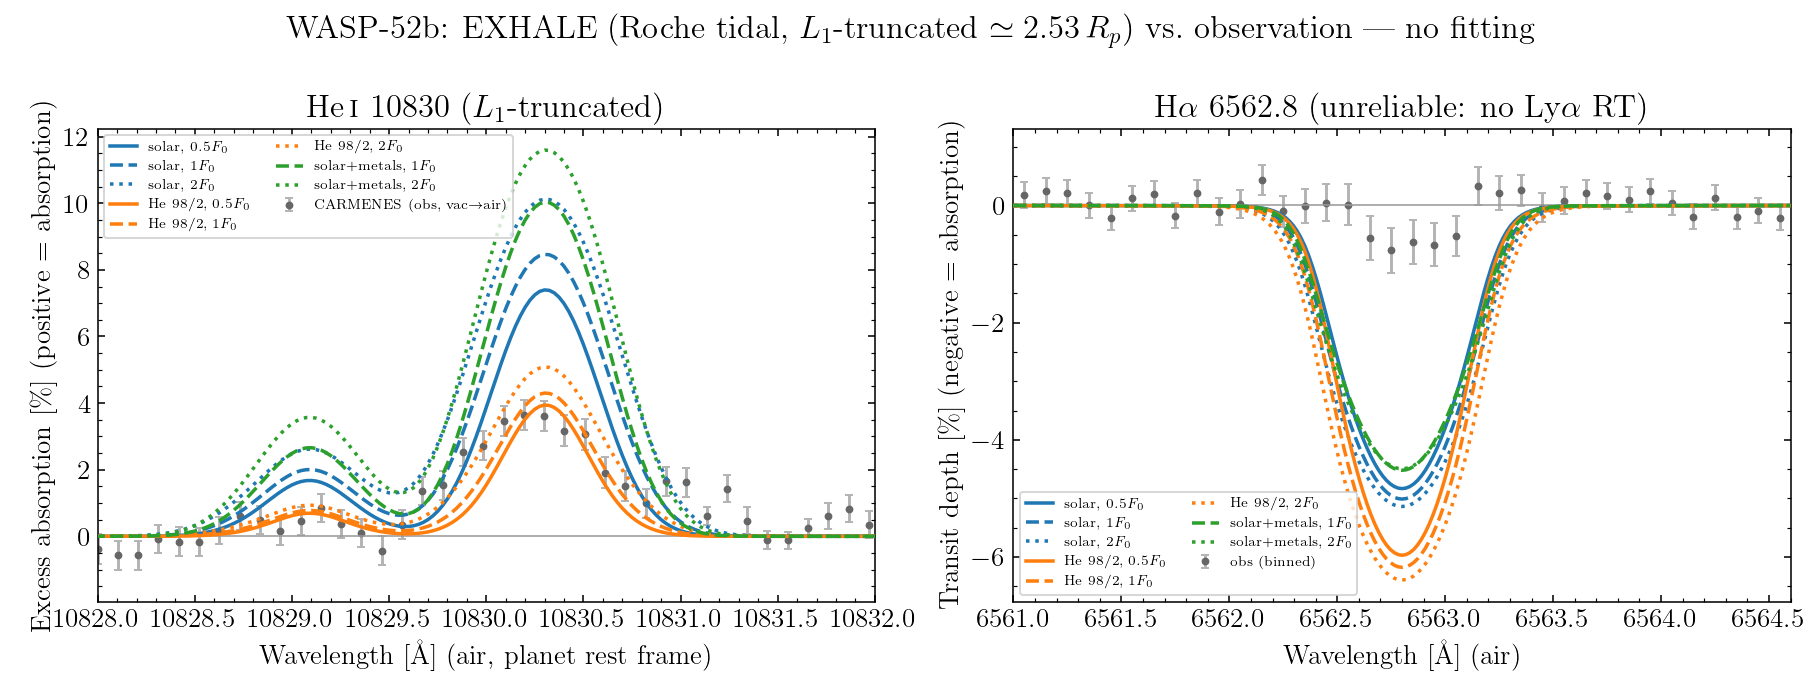
\includegraphics[width=\textwidth]{compare_WASP-52b_L1.png}
\caption{$L_1$-truncated ($\simeq2.53\,\Rp$) model vs.\ observations, same layout
as Fig.~\ref{fig:cmp10rp}. The He-poor $0.5\,\Fo$ model (orange solid) matches the
observed He\,10830 line. H$\alpha$ (right) is shown for completeness only.}
\label{fig:cmpL1}
\end{figure}

\begin{figure}[h]
\centering
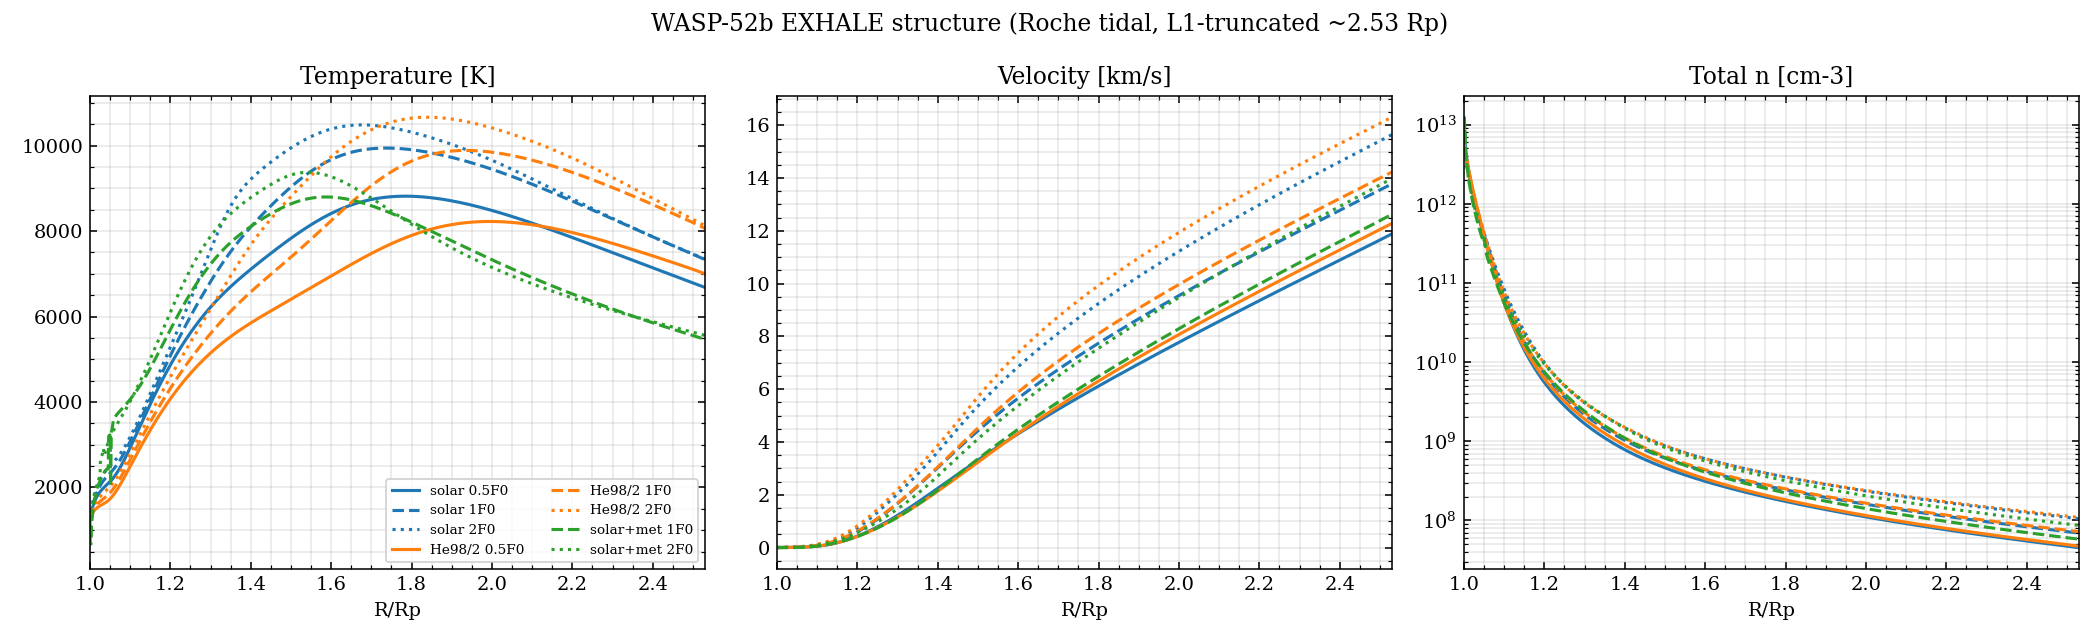
\includegraphics[width=\textwidth]{profiles_WASP-52b_L1.png}
\caption{Converged atmospheric structure (temperature, velocity, total number
density) for the $L_1$-truncated runs. Color $=$ composition, line style $=$ XUV
level.}
\label{fig:profL1}
\end{figure}

\section{H/He scan}
\label{sec:scan}
To locate the composition that matches the He\,10830 line we scan the He/H number
ratio from solar (92/8) to strongly He-poor (99.5/0.5) at the best-fit flux
($0.5\,\Fo$) in the $L_1$-truncated domain (Table~\ref{tab:scan},
Fig.~\ref{fig:scan}). The He\,10830 excess absorption decreases monotonically with
decreasing He/H, from $7.4\%$ (solar) to $1.5\%$ (99.5/0.5). The observed depth
($\sim$3.4\%) is bracketed by H/He $=$ 98/2 ($3.9\%$) and 99/1 ($2.5\%$), implying a
best-fit ratio of H/He\,$\approx$\,98.3/1.7 (He/H\,$\approx$\,0.017). This is a
strongly He-depleted atmosphere relative to solar, in line with the high H/He ratio
that Yan et al.\ (2022) required to reproduce the He\,10830 line.

\begin{table}[h]
\centering
\caption{He\,10830 line-center excess absorption [\%] vs.\ composition, at
$0.5\,\Fo$ in the $L_1$-truncated domain. Observed $\sim$3.4\%.}
\label{tab:scan}
\begin{tabular}{lll}
\toprule
He/H & H/He & He\,10830 [\%] \\
\midrule
0.087 & 92/8 (solar) & 7.40 \\
0.050 & 95.2/4.8     & 6.04 \\
0.020 & 98/2         & \textbf{3.94} \\
0.010 & 99/1         & 2.52 \\
0.005 & 99.5/0.5     & 1.47 \\
\bottomrule
\end{tabular}
\end{table}

\begin{figure}[h]
\centering
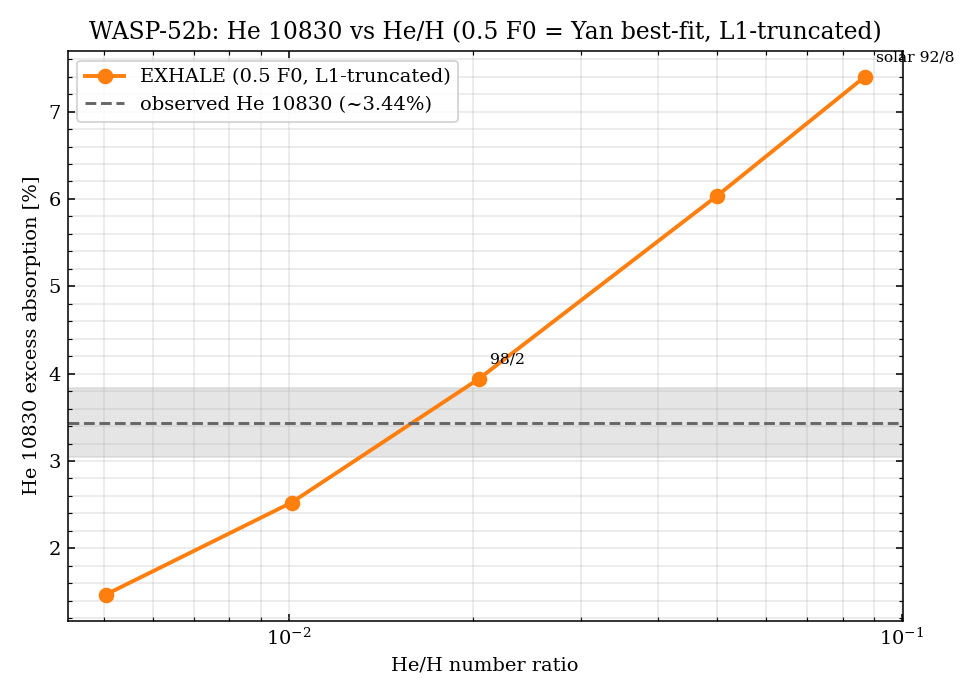
\includegraphics[width=0.72\textwidth]{hescan_WASP-52b.png}
\caption{He\,10830 excess absorption vs.\ He/H number ratio ($0.5\,\Fo$,
$L_1$-truncated). The dashed line and gray band are the observed depth
($3.44\pm0.4\%$). The model crosses the observation near H/He\,$\approx$\,98/2,
confirming the need for a He-depleted atmosphere.}
\label{fig:scan}
\end{figure}

\section{H$\alpha$ caveat}
\label{sec:halpha}
The H$\alpha$ line absorbs from the $n=2$ hydrogen population, which is set
primarily by Ly$\alpha$ radiative pumping. \texttt{EXHALE}/\texttt{TPM.py} estimate
the Ly$\alpha$ mean intensity with the simple Huang et al.\ (2017) prescription
rather than a full Ly$\alpha$ radiative-transfer solution. The resulting $n=2$
population, and hence the H$\alpha$ prediction, is therefore not reliable and is
shown in the figures for completeness only. A proper Ly$\alpha$ RT treatment is
required before the H$\alpha$ comparison can be interpreted.

\section{Conclusions}
\begin{enumerate}
\item \texttt{EXHALE} reproduces the Yan et al.\ (2022) steady-state mass-loss
  rates at every XUV flux to within $\sim$10\% (Table~\ref{tab:mdot}).
\item The He\,10830 line depth is controlled by the metastable $\HeTS$ population.
  An extended $10\,\Rp$ domain over-predicts the absorption by $3$--$10\times$
  because the outer $\HeTS$ tail beyond $L_1$ dominates the impact-parameter
  integral; the bound atmosphere ($r<L_1$) alone gives the observed depth.
\item With the $L_1$-truncated domain, a He-poor composition (H/He\,$\simeq$\,98/2)
  and the best-fit flux ($0.5\,\Fo$), the model reproduces the observed He\,10830
  line ($\sim$3.9\% vs.\ $\sim$3.4\%), independently confirming Yan's requirement
  of a high H/He ratio.
\item H$\alpha$ is not modeled reliably here because the Ly$\alpha$ radiative
  transfer is not solved.
\end{enumerate}

\section*{References}
\begingroup
\setlength{\parindent}{0pt}\setlength{\parskip}{4pt}
\everypar{\hangindent=1.5em\hangafter=1}
Caldiroli, A., Haardt, F., Gallo, E., et al.\ 2021, A\&A, 655, A30.
``Irradiation-driven escape of primordial planetary atmospheres.~I. The ATES
photoionization hydrodynamics code.''

Erkaev, N.~V., Kulikov, Yu.~N., Lammer, H., et al.\ 2007, A\&A, 472, 329.
``Roche lobe effects on the atmospheric loss from hot Jupiters.''

France, K., Loyd, R.~O.~P., Youngblood, A., et al.\ 2016, ApJ, 820, 89.
``The MUSCLES Treasury Survey.~I.''

Huang, C., Arras, P., Christie, D., \& Li, Z.-Y. 2017, ApJ, 851, 150.
``A Model of the H$\alpha$ and Na Transmission Spectrum of HD\,189733b.''

Yan, D., Seon, K.-i., Guo, J., Chen, G., \& Li, L. 2022, ApJ, 936, 177.
``Modeling the H$\alpha$ and He\,10830 Transmission Spectrum of WASP-52b.''

Yang, L., \& Guo, J. 2018, RAA, 18, 077 (arXiv:1806.04719).
``Effect of Orbital Distance on the Atmospheric Escape of Exoplanets.''
\endgroup

\end{document}
